%======================================================================
%  Common part of the three guides: method, blocks, figures, values
%======================================================================
\sessiontitle{Chapter 3 -- Reciprocity: the three codes}
  {Common to the Cast3M, FEniCS and Python guides that follow.}

\guidesec{1\quad Purpose}
The three files \texttt{rg\_session.dgibi} (Cast3M),
\texttt{rg\_session\_fenics.py} (FEniCS) and \texttt{rg\_session.py} (Python,
scikit-fem) do the same computation, block by block. They compute the
Cauchy data of a cracked rectangle, form reciprocity gaps with the four
families of adjoint fields of the session sheet, and identify the crack.
They start from the files of the author: the Cast3M procedure
\texttt{crack\_rg\_extension.dgibi} (version 3, Cast3M 2026), its Python
replica (\texttt{replica.py}, gmsh + scikit-fem) and the FEniCS script
\texttt{reciprocity\_gap\_crack.py} (DOLFINx + gmsh). The geometry, the
mesh of the replica, the discrete gap with the nodal fluxes $\mat Ku$ and the
measurement procedure are kept; the comments are in English and the
blocks are the same in the three files.

\guidesec{2\quad Method in one page}
In $\Omega=(0,\ell)\times(0,h)$ with an insulated crack $\Gamma$, $u$ is
harmonic in $\Omega\setminus\Gamma$ with $\partial_nu=0$ on both lips. For any
$v$ harmonic in the whole of $\Omega$,
\[
\RG(v)=\int_{\partial\Omega}\bigl(u\,\partial_\nu v-v\,\varphi\bigr)\dd s
=\int_\Gamma\jump u\,\partial_nv\dd s,\qquad\varphi=\partial_\nu u .
\]
The files evaluate it with nodal values on the boundary,
$\RG_h(v)=\vect U_b\cdot(\mat K\vect V)_b-\vect Q_b\cdot\vect V_b$, with $\mat K$
the conductivity matrix and $\vect Q=\mat K\vect U$ the nodal fluxes. This is
the sign of the notes; the file \texttt{crack\_rg\_extension.dgibi} uses the
opposite sign, which cancels in all ratios. For the harmonic polynomials of
degree $\le2$ the identity is exact with quadratic elements (sheet,
question a.5). With $\vect X=\vx-\vx_0$, $s=\vt\cdot\vect X$,
$\eta=\vn\cdot\vect X-c$ and $s'=s-s_0$:
\begin{center}\small
\renewcommand{\arraystretch}{1.15}
\begin{tabular}{llll}
\toprule
\sffamily block & \sffamily adjoint field $v$ & \sffamily $\RG(v)$ & \sffamily gives\\
\midrule
6 & $X$, $Y$ & $m_0n_x$, $m_0n_y$ & normal $\vn$, signal $m_0$\\
6 & $(\vn\cdot\vect X)^2-(\vt\cdot\vect X)^2$ & $2c\,m_0$ & line $\vn\cdot\vect X=c$\\
7 & $\eta$, $s\eta$, $s'^2\eta-\eta^3/3$ & $m_0$, $m_0s_0$, $m_0\mu_2$ & centre $s_0$, $a_{\rm mom}=2\sqrt{\mu_2}$\\
7 & (dipole) & $m_0=\pi a^2E_n$ & $a_{\rm dip}=\sqrt{m_0/(\pi E_n)}$\\
8 & $e^{\xi\eta}\cos\xi s'$, $e^{\xi\eta}\sin\xi s'$ & $\xi C(\xi)$, $\xi S(\xi)$ & $C/m_0=2J_1(\xi a)/(\xi a)$, $S=0$\\
8 & $\sin(\lambda_kg)\sinh(\lambda_k\eta)/\lambda_k$ & sine coefficients & $w(g)$, series\\
9 & $X$, $Y$ for 12 angles & rows of $R=\vm\vn^\top$ & $\vn$, $\vm$, virtual experiment\\
\bottomrule
\end{tabular}
\end{center}
Experiment E1 has electrodes at the bottom ($u=0$) and top ($u=h$), field
$\vE=(0,1)$. The turning potential imposes $u=\vd_\beta\cdot\vect X$ on the
whole boundary, field $\vd_\beta$, and measures only the flux; by linearity
two solves give all the angles.

\guidesec{3\quad The blocks (same in the three files)}
\begin{center}\small
\renewcommand{\arraystretch}{1.1}
\begin{tabular}{>{\sffamily}l p{6.4cm} p{5.6cm}}
\toprule
block & content & output\\
\midrule
0 & parameters (table in each guide) & \\
1 & geometry and mesh, two lips & \\
2 & model, conductivity matrix, centred coordinates $\vect X$ & FIG 1\\
3 & procedures: gap \texttt{rgap}, measurement \texttt{measure}/\texttt{mesbr}, opening & \\
4 & experiment E1, opening $\jump{u_1}$ read on the lips & FIG 2, FIG 3\\
5 & measurement with noise, $\RG(1)$ & \\
6 & linear and quadratic fields: $\vn$, $c$ & \\
7 & polynomial fields: $m_0$, $s_0$, $\mu_2$, lengths; dipole & FIG 4, FIG 5\\
8 & Fourier fields $C(\xi)$, $S(\xi)$, Fourier length; sine--sinh series & FIG 6, FIG 7\\
9 & turning potential, matrix $R$, its rank one, virtual experiment & FIG 8, FIG 9\\
\bottomrule
\end{tabular}
\end{center}
The procedures differ only in syntax. \texttt{rgap(ub, qb, v)} returns
$\RG_h(v)$ from the boundary values; \texttt{measure} (\texttt{mesbr} in
gibiane) returns the Cauchy data on the boundary with an independent,
multiplicative Gaussian noise of level \texttt{eps} on the measured values
only ($u$ where the flux is imposed, the flux where $u$ is imposed, never
$u$ at the corners).

\guidesec{4\quad The figures: what is what}
The title of each plot starts with its number (\texttt{FIG k}), and a message
explaining it is printed just before. The figures below were produced by
the Python file at \texttt{eps = 0}; the FEniCS file uses the same mesh and
gives the same figures; Cast3M draws them in its own style.

\begin{center}
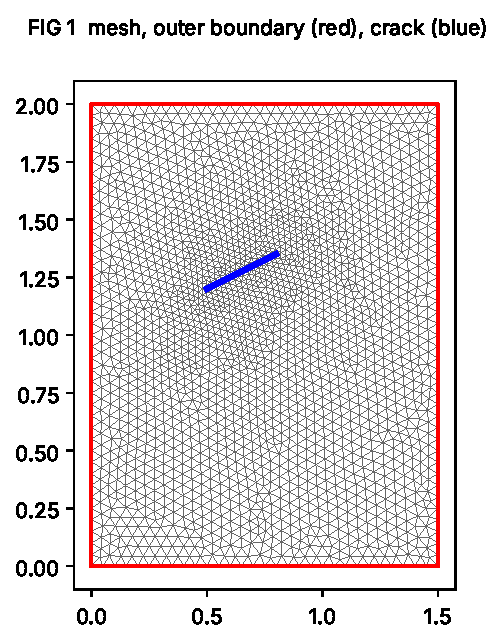
\includegraphics[height=4.6cm]{ch3/figs/python/fig1}\hfill
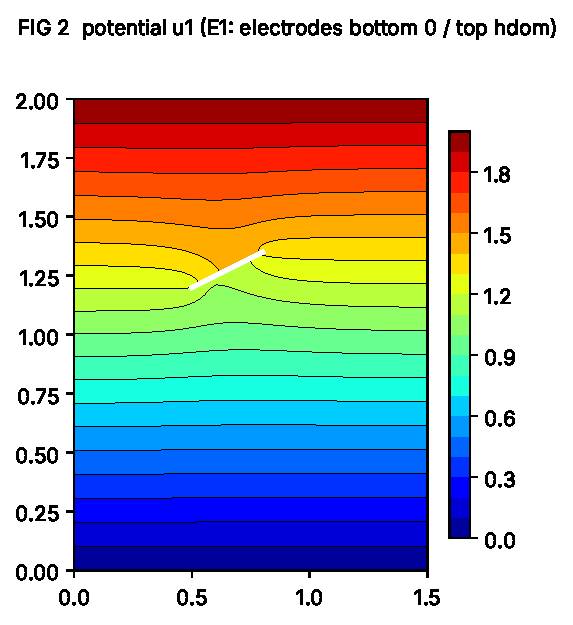
\includegraphics[height=4.6cm]{ch3/figs/python/fig2}\hfill
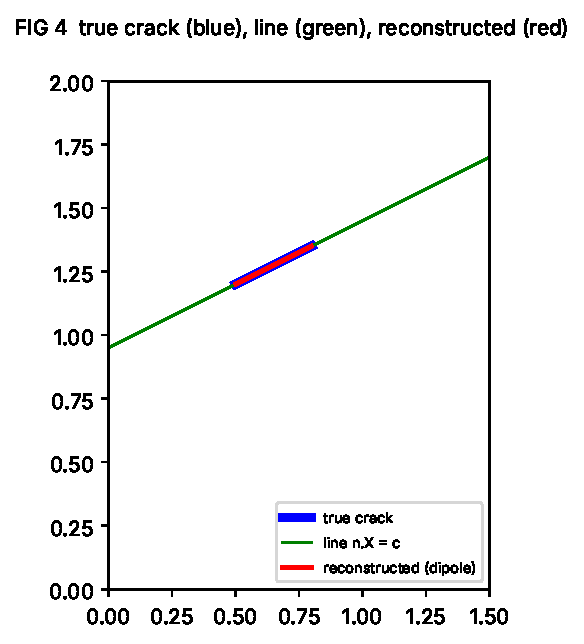
\includegraphics[height=4.2cm]{ch3/figs/python/fig4}
\end{center}
\textbf{FIG 1 -- mesh.} Red: outer boundary, where the data are measured;
blue: the crack, whose nodes are doubled (two lips). The mesh is refined at
the crack (size $\ell_\Gamma/15$) and has size $\ell/30$ elsewhere.
\textbf{FIG 2 -- potential $u_1$.} Far from the crack the isolines are
straight (the field $(0,1)$); near the crack they are bent and crowd at the
tips, since no current crosses it. \textbf{FIG 4 -- identified crack.} Blue:
true crack; green: line $\vn\cdot\vect X=c$ (Block 6); red: reconstructed
segment $\vx_0+c\vn+(s_0\pm a_{\rm dip})\vt$ (Block 7). Without noise red covers
blue.

\begin{center}
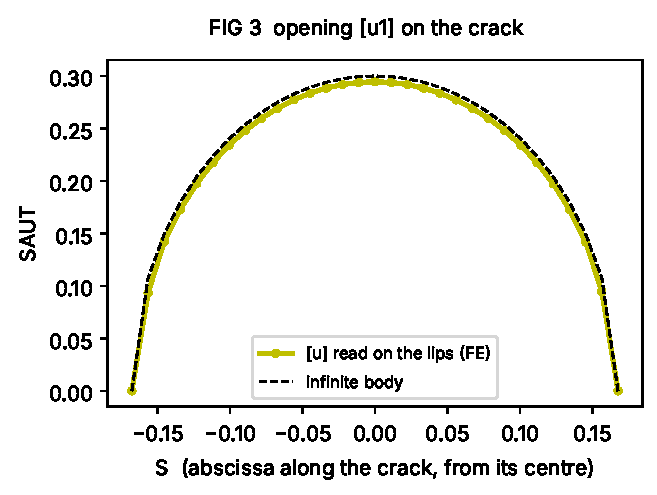
\includegraphics[width=0.32\textwidth]{ch3/figs/python/fig3}\hfill
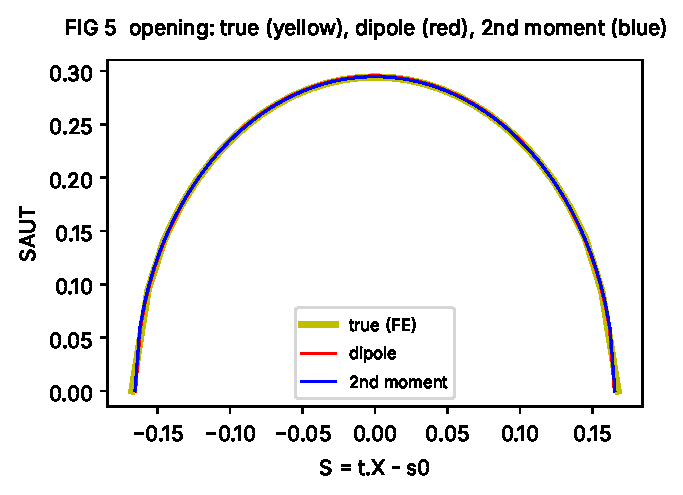
\includegraphics[width=0.32\textwidth]{ch3/figs/python/fig5}\hfill
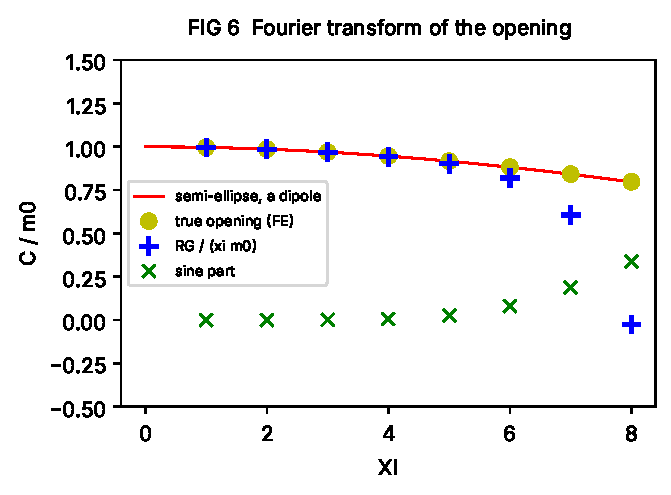
\includegraphics[width=0.32\textwidth]{ch3/figs/python/fig6}
\end{center}
\textbf{FIG 3 -- opening $\jump{u_1}$} read on the doubled nodes, against the
infinite-body opening $2E_n\sqrt{a^2-s^2}$ (dashed), slightly larger.
\textbf{FIG 5 -- opening and reconstructions.} Yellow: true opening;
red: semi-ellipse of area $m_0$ and half-length $a_{\rm dip}$; blue: the same
with $a_{\rm mom}$ (drawn only if $\mu_2>0$). Without noise they coincide; with
noise blue moves first. \textbf{FIG 6 -- Fourier transform.} Red:
$2J_1(\xi a)/(\xi a)$ with $a=a_{\rm dip}$; yellow: $C/m_0$ of the true
opening; blue crosses: $\RG/(\xi m_0)$; green: the sine part $S/m_0$, which
should vanish. Crosses leave the curve, and green leaves $0$, from
$\xi\approx5$.

\begin{center}
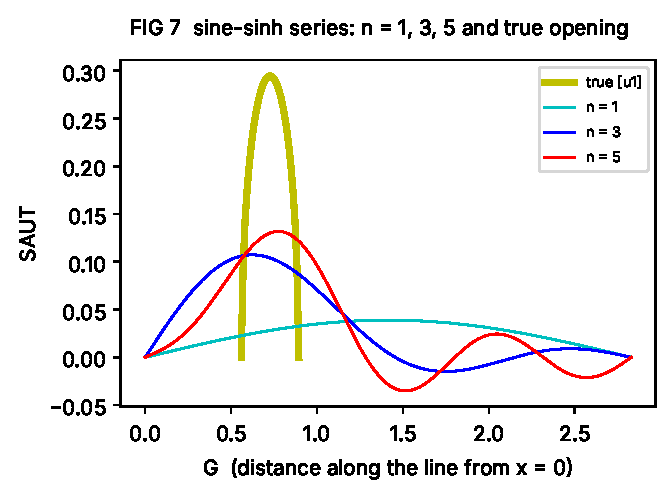
\includegraphics[width=0.32\textwidth]{ch3/figs/python/fig7}\hfill
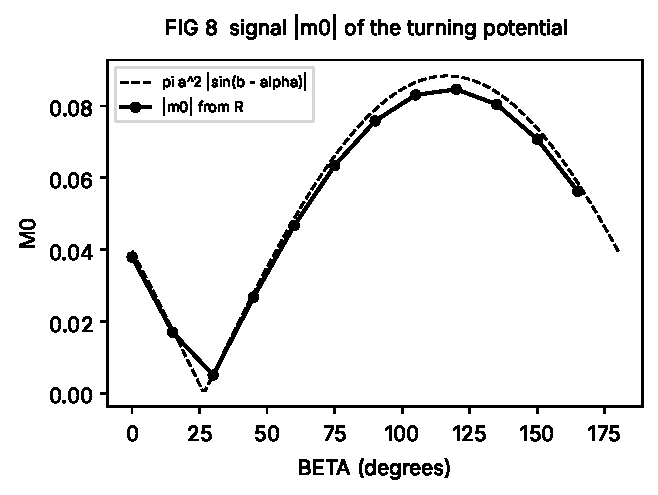
\includegraphics[width=0.32\textwidth]{ch3/figs/python/fig8}\hfill
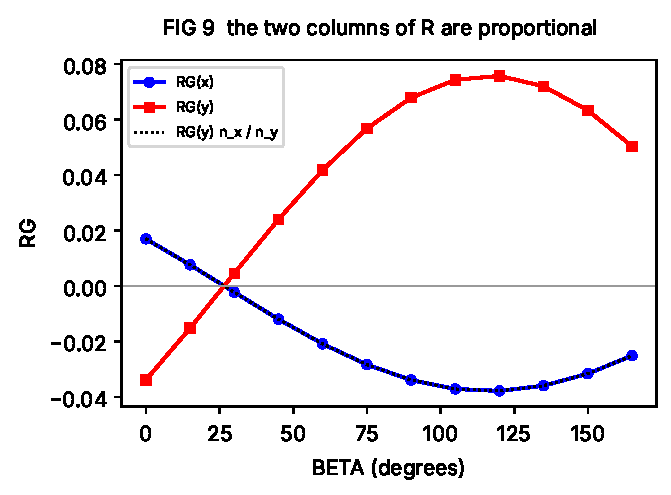
\includegraphics[width=0.32\textwidth]{ch3/figs/python/fig9}
\end{center}
\textbf{FIG 7 -- sine--sinh series.} Abscissa $g$ from the point of the line
at $x=0$, $L=\sqrt2\max(\ell,h)=2.83$; yellow: true opening; partial sums
$n=1,3,5$. The terms resolve details of size $L/n\gtrsim0.5$, larger than the
crack, and the high terms carry the discretization error.
\textbf{FIG 8 -- signal of the turning potential.} $|m_0|$ against $\beta$,
with $\pi a^2|\sin(\beta-\alpha)|$ (dashed): zero for the field parallel to
the crack ($\alpha=26.6^\circ$), largest for the normal field.
\textbf{FIG 9 -- the columns of $R$.} $\RG(X)$ and $\RG(Y)$ against $\beta$:
proportional, in the ratio $n_x/n_y$ (dotted, on top of the blue curve).

\guidesec{5\quad Reference values}
Python and FEniCS (same gmsh mesh: 4242 triangles, 8654 nodes, P2) at
\texttt{eps = 0}. True crack: $\vn=(-0.4472,0.8944)$, $c=0.2907$, length
$0.3354$, centre $(0.65,1.275)$. Cast3M, on its own mesh, should agree to
about two digits.
\begin{center}\small
\renewcommand{\arraystretch}{1.1}
\begin{tabular}{>{\sffamily}l l l}
\toprule
block & message & value\\
\midrule
4 & \texttt{int [u] on the lips} (infinite body) & 0.07641 (0.07903)\\
5 & \texttt{RG(1)} & $\approx10^{-13}$\\
6 & \texttt{RG(x)}, \texttt{RG(y)} & $-0.03427$, $0.06855$\\
6 & \texttt{normal n}, \texttt{angle error} & $(-0.4472, 0.8944)$, $0.0000^\circ$\\
6 & \texttt{line c} & 0.2907\\
7 & \texttt{m0}, \texttt{s0}, \texttt{mu2}, \texttt{E\_n} & 0.07664, $-0.0336$, 0.006855, 0.8944\\
7 & \texttt{length (2nd moment)}, \texttt{(dipole)} & 0.3312, 0.3303 (tip error 0.0026)\\
8 & $C/m_0$ at $\xi=1,2,3,4$ & 0.9966, 0.9864, 0.9691, 0.9428\\
8 & \texttt{length (Fourier, xi = 2)} & 0.3306\\
8 & sine--sinh \texttt{RG\_k}, $k=1..5$ & $-0.0551$, $-0.0753$, $-0.0487$, 0.0051, 0.0467\\
9 & singular values of $R$ & 0.20767, $\approx10^{-13}$\\
9 & $|m_0|$ min / max & 0.0051 at $30^\circ$ / 0.0846 at $120^\circ$\\
9 & virtual field $\vd_{\rm v}$, $c$, length & $(-1.0954, 2.1909)$, 0.2907, 0.3285\\
\bottomrule
\end{tabular}
\end{center}
With noise each run draws new numbers (Python and FEniCS: change
\texttt{seed}). Over 200 draws for E1: at $\texttt{eps}=10^{-3}$, dipole length
$0.330\pm0.001$, second-moment length $0.325\pm0.078$ (3 failures,
$\mu_2\le0$); at $10^{-2}$, $0.331\pm0.010$ and $0.61\pm0.25$ (81 failures).
